\begin{frame}{Villeneuve-la-Garenne}
  \footnotesize
  En groupes de 4, lisez à tour de rôle \gloss{taking turns} le texte qui commence à la page 85 du manuel.
  Après chaque paragraphe, répondez aux questions suivantes et discutez-en.
  \begin{center}
    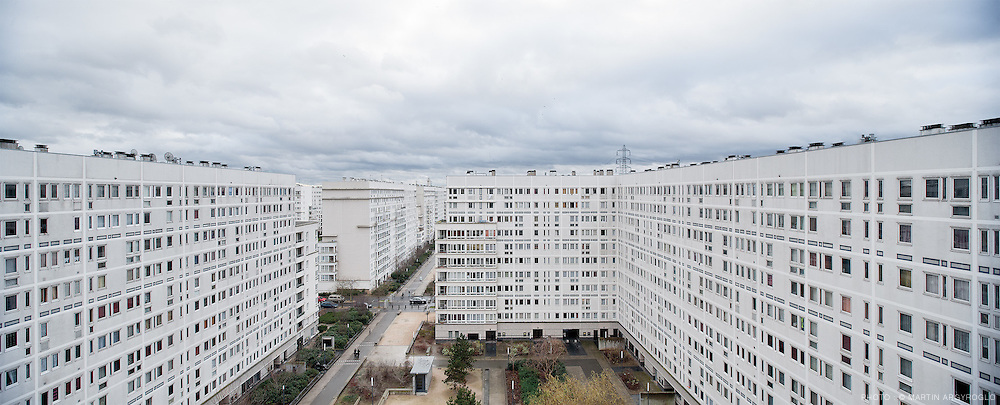
\includegraphics[scale=0.75]{caravelle.jpg}
  \end{center}
  \begin{itemize}
    \item (L1-L7) Est-ce que la Caravelle est belle? Quelle partie du texte te l'indique?
    \item (L8-L16) Quels sont les emplois de Kamel, Abdoul Razak et Medhi?
    \item (L17-L23) Comment Kamel a-t-il enfin réussi à obtenir un entretien?
    \item (L24-L35) Est-ce que Abdoul Razak et Medhi ont l'air optimiste ou pessimiste? Comment le savez-vous?
    \item (L36-L39) Quelle est la différence entre les gens de ce HLM qui ont des diplômes et ceux qui n'en ont pas?
    \item (L40-L47) Qui est ``Mathieu'', et pourquoi Nadir en parle-t-il?
  \end{itemize}
\end{frame}